\documentclass[hyperref={colorlinks = true,linkcolor = blue, citecolor = blue, urlcolor = blue}]{beamer}

\setbeamertemplate{navigation symbols}{}
\setbeamertemplate{footline}[frame number]
 
\usepackage[utf8]{inputenc}

\usepackage[newfloat]{minted}

\usepackage{pgf}
\usepackage{tikz}
\usepackage{upquote}
\usepackage{natbib}
\usepackage{graphicx}

\usetikzlibrary{arrows,automata}
\bibliographystyle{abbrvnat}
\graphicspath{{./images/}}

\newenvironment{code}{\captionsetup{type=listing}}{}
\SetupFloatingEnvironment{listing}{name=Listing}

\title{Russel vs Tarski Universes}
\author{Donovan Crichton}
\date{August 2022}

\begin{document}
 
\frame{\titlepage}

\begin{frame}[fragile]
  \frametitle{Preliminaries}
  \begin{itemize}
  \item Slides and Examples available at:
    \url{https://github.com/donovancrichton/ANU-TT}
  \item This talk: /RusselVsTarskiUniverses
  \end{itemize}
\end{frame}

\begin{frame}[fragile]
\frametitle{Origin - Per Martin-L{\"o}f}
\citep[p. 87-91]{martin1984intuitionistic}
\begin{center}
  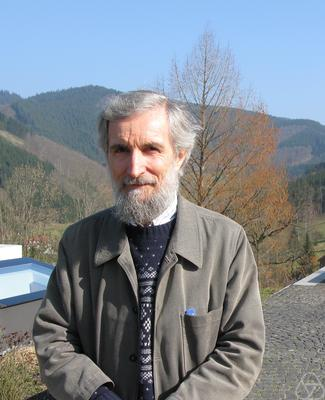
\includegraphics[scale=0.5]{PerMartinLof}
\end{center}
\end{frame}

\begin{frame}[fragile]
\frametitle{Transfinite Types}
  \begin{itemize}
    \item MLTT has \mintinline{idris}{Type : Type}.
    \item Martin-L{\"o}f introduces Universes to allow transfinite type formers.
    \item Without Universes we have Girard's Paradox \citet{girard1972interpretation}.
  \end{itemize}
\end{frame}

\begin{frame}[fragile]
  \frametitle{Unsoundness in Idris from \mintinline{idris}{Type : Type}}
  \begin{itemize}
    \item Hurken provides us with a simpler proof based around Burali-Forti's
          Paradox \citet{hurkens1995simplification}. 
    \item Apparently this encoding represents well-orderings/well-foundedness...
          I don't see it!
    \item Let's see the \href{https://github.com/donovancrichton/ANU-TT/blob/master/RusselVsTarskiUniverses/Code/src/HurkensParadoxLoop.idr}{code}.
  \end{itemize}
\end{frame}

\begin{frame}[fragile]
\frametitle{References}
\bibliography{references}{}
\end{frame}


\end{document}

